\section{Introduction}


In Chapter \ref{ch:ReactionModels} we have established that our "Symmetric" and "Asymmetric" HDAC6 complex formation models are capable of predicting capsid breakage in normal and perturbed conditions. Our next point of interest is to try and use them to make predictions for cases for which we don't know the answer for.

One possible application has been suggested by the data provided by our collaborators from Patrick Matthias' group at FMI. They used designed ankyrin repeat proteins (DARPins) - artificial proteins which can bind target proteins with high affinity and specificity - to try and find one capable of inhibiting HDAC6-mediated influenza uncoating.

To  compare our experimental DARPin-F10 data and our dose-response predictions we sought out existing influenza infection models. Non-structured \textit{in vitro} influenza kinetic models were considered a good fit for our goals, as they mostly rely on directly observed experimental quantities such as viral growth.

Some of the newer studies describing structured and non-structured kinetic models \cite{rudiger2019multiscale, schulze2009infection} use attractive multi-dimensional datasets, which even without the use of the model may allow predictions of infection progression. Such datasets, when available, provide an intriguing opportunity to functionally characterise influenza infection, and make corresponding adjustments in our model structure.

For example, it has long been established that higher MOI tends to lead to higher synchrony of viral release \cite{cairns1957asynchrony}. Influenza kinetic models tend to implicitly build it into the parameter fitting. However, if the fitting datset only includes a small variety of initial conditions, specifically with regard to initial virus concentration, it is difficult to judge how well the model would describe any other dataset.

In this chapter we give a brief summary of experimental data available for DAPin-F10 \cite{DarpinData}, provide an overview on \textit{in vitro} influenza kinetic modelling literature, make predictions about DARPin-F10 active concentrations and dose-response behavior, make use of available literature data \cite{rudiger2019multiscale, schulze2009infection} to analyze functional dependencies between model parameters, and to fit a simple influenza infection model, which we then attempt to use in conjunction with the predicted DARPin-F10 dose response.

\subsection{DARPin-F10 inhibits HDAC6-ZnF Ub binding}

\begin{figure}
\begin{center}
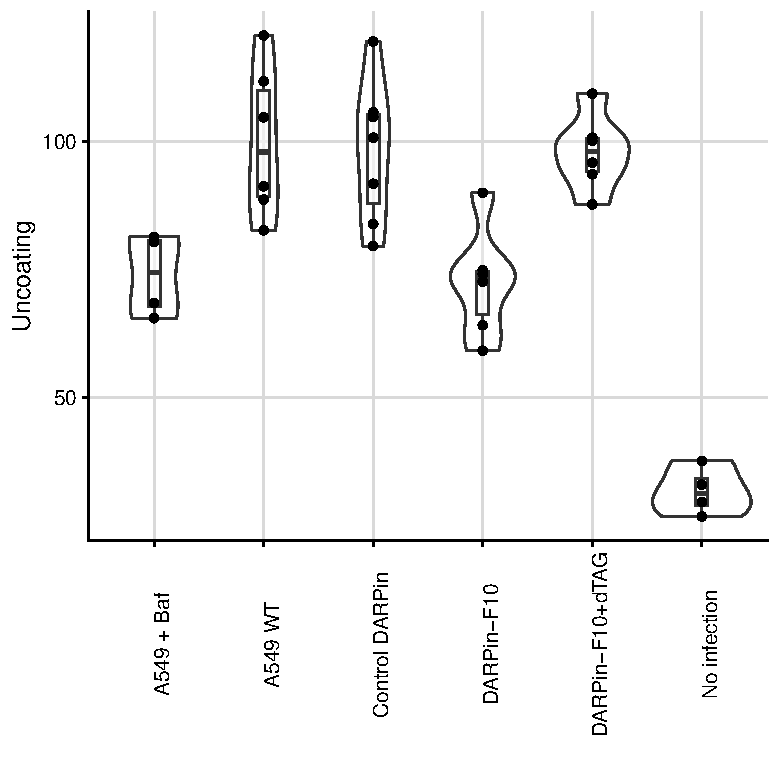
\includegraphics[width=0.95\textwidth, trim={0cm 0cm 0cm 0cm}, clip]{D_chapters/3_DARPinModels/DarpinUncoating.pdf}
\caption[DARPin-F10 reduces influenza virus uncoating]%
{DARPin-F10 at MOI = 30 PFU/ml reduces influenza virus uncoating\par
A549 + Baf: the cells treated with Bafilomycin, an ATPase inhibitor which also stops viral uncoating;\par
A549 WT: wild type;\par
CTR DARPin: cells with a DARPin that did not bind anything;\par
DARPin-F10: cells with a DARPin that binds HDAC6 ZnF;\par
DARPin-F10 + dTAG: cells in which DARPin F10 was degraded through dTAG before virus infection;\par
* No infection: cells without any virus added to them.\par
All the values are normalized to A549 WT.}
\label{figure:darpinUncoatingExperimental}
\end{center}
\end{figure}

\begin{figure}
\begin{center}
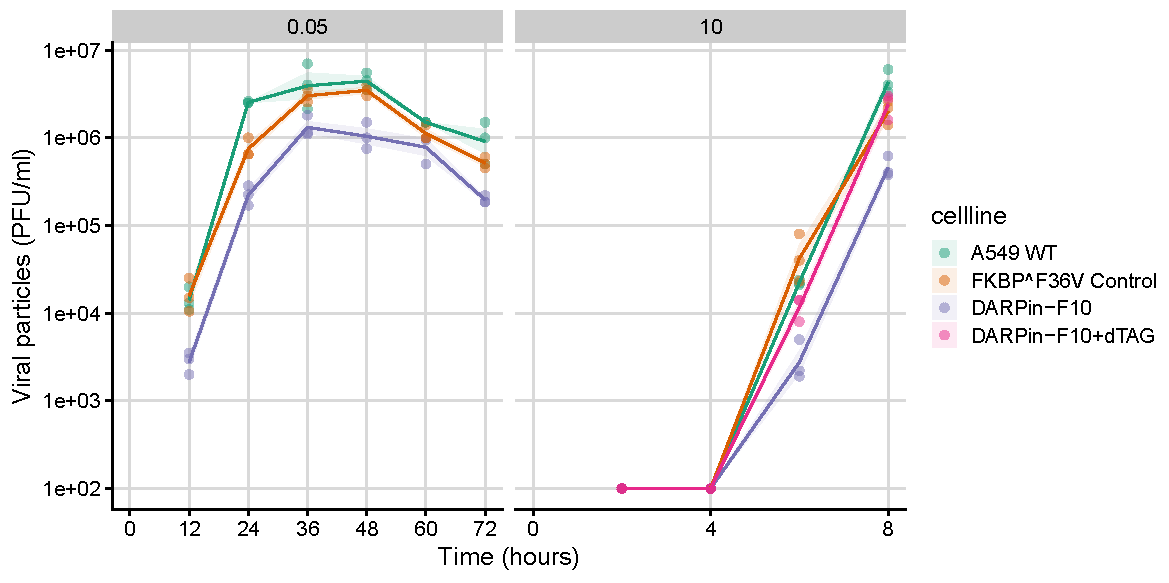
\includegraphics[width=0.95\textwidth, trim={0cm 0cm 0cm 0cm}, clip]{D_chapters/3_DARPinModels/DarpinVirusProduction.pdf}
\caption[DARPin-F10 reduces viral growth]%
{DARPin-F10 at MOI = 0.05 and 10 PFU/ml reduces viral growth\par
A549 WT: wild type;\par
FKBP\textasciicircum F36V Control: cell line with a different mutation.\par
DARPin-F10: cells with a DARPin that binds HDAC6 ZnF;\par
DARPin-F10 + dTAG: cells in which DARPin F10 was degraded through dTAG before virus infection.}
\label{figure:darpinGrowthExperimental}
\end{center}
\end{figure}

Our collaborators from Patrick Matthias’ group at FMI showed that DARPin-F10 has a high specificity and affinity against HDAC6-ZnF \cite{DarpinData}. They were able to stably express and reversibly DARPin F10 in A549 cells. Using these new mutant cell lines they demonstrated that at multiplicity of infection (MOI) of 30 plaque-forming units (PFU) /ml DARPin-F10 expression leads to the reduction in influenza viral uncoating (Figure \ref{figure:darpinUncoatingExperimental}), and at MOIs of 10 and 0.05 PFU/ml - to reduction virus production (Figure \ref{figure:darpinGrowthExperimental}).

Knowing that DARPin-F10 binds to HDAC6-ZnF we can with reasonably assume that during influenza uncoating it acts as a competitor against polyubiquitin chains. In this chapter, we use that assumption, and introduce DARPin-F10 to our HDAC6 complex formation models.

\subsection{Influenza infection modelling}

Seasonal and zoonotic influenza is a popular subject of viral modelling, which has a variety of approaches. Majority of viral models use systems of ordinary differential equations (ODE), but partial (PDE) and delay differential equations (DDE) have also been implemented.

Influenza infection dynamic models are focused primarily capturing the transmission between hosts, with the goal of informing public health decisions an assist in pandemic planning \cite{ferguson2006strategies, mcvernon2007model}.

With the advancement of the social media, a new type of influenza forecasting models has emerged \cite{pawelek2014modeling, santillana2015combining}, relying on publicly available self-reporting by users.

Structured models which include individual processes in virus replication \cite{sidorenko2004structured}, endosomal escape \cite{lagache2012modeling} and defective viral particle propagation \cite{rudiger2019multiscale} have been proposed. Their phenomenological nature means that they often rely on unobserved quantities and variables, and often don't allow for inference on specific molecular targets for intervention.

Non-structured influenza kinetic models aim to understand and quantify severity, duration, and overall progression of the infection within a host or a cell culture. \textit{In vitro} models usually have a simple and understandable structure, and rely on directly observed experimental quantities. \textit{In vivo} kinetic models usually build up on that basic structure and attempt to incorporate innate \cite{beauchemin2008modeling} and adaptive \cite{belz2002compromised} immune response. Here we primarily focus on \textit{in vitro} models, as our DARPin-F10 experimental data is coming from cell culture experiments.

Chronic infection kinetic model, originally proposed for human immunodeficiency virus (HIV) \cite{perelson2002modelling}, includes three states: $T$ - target cells, $I$ - infected cells, $V$ - viral particles, which are described as follows:

\begin{equation}
\begin{array}{rcl}
\frac{dT}{dt} &=& s T - d T - \beta T V \\
\frac{dI}{dt} &=& \beta T V - \delta I \\
\frac{dV}{dt} &=& p I - c V
\end{array}
\end{equation}

where $s$ is target cells regeneration, $d$ is natural target cells death, $\beta$ is target cells infection rate by viral particles, $\delta$ is death rate of infected cells, $p$ is viral particle production rate by infected cells, and $c$ is clearance rate of viral particles.

It's often assumed that during acute ($s = d = 0$ \cite{baccam2006kinetics}) influenza infection target cells $T$ are limited and are depleted over the course of the infection:

\begin{equation}
\begin{array}{rcl}
\frac{dT}{dt} &=& - \beta T V \\
\frac{dI}{dt} &=& \beta T V - \delta I \\
\frac{dV}{dt} &=& p I - c V
\end{array}
\end{equation}

Another commonly made assumption is that during influenza infection viral production is delayed, which is accomplished through presence of a latent eclipse phase infected cells $I_1$ and productively infected cells $I_2$ (\cite{baccam2006kinetics}):

\begin{equation}
\begin{array}{rcl}
\frac{dT}{dt} &=& - \beta T V \\
\frac{dI_1}{dt} &=& \beta T V - k I_1 \\
\frac{dI_2}{dt} &=& k I_1 - \delta I_2 \\
\frac{dV}{dt} &=& p I_2 - c V
\end{array}
\end{equation}

where $k$ is a rate of $I_1$ maturation into $I_2$.

Alternative approach to modeling this latency is through introducing a fixed delay $\tau$:

\begin{equation}
\begin{array}{rcl}
&\frac{dT}{dt} = - \beta T(t) V(t) \\
&\frac{dI}{dt} = \beta T(t-\tau) V(t-\tau) - \delta I(t) \\
&\frac{dV}{dt} = p I(t) - c V(t)
\end{array}
\end{equation}

Here, "eclipse phase" the infected cell doesn't contribute to systems dynamics. Delay model disregards variability of transition time from eclipse phase, but allows to avoid unrealistically small or large transition times from eclipse to productive phase \cite{beauchemin2008modeling}.

\cite{mohler2005mathematical,schulze2009infection} model viral production on microcarriers and introduce delay in viral production term $p I(t - \tau)$ instead.

Several models have been suggested to describe influenza infection in presence of antiviral drugs. Amantadine drugs are commonly modelled as follows:

\begin{equation}
\begin{array}{rcl}
\frac{dT}{dt} &=& - (1-\epsilon_{drug})\beta T V \\
\frac{dI}{dt} &=& \beta T V - \delta I \\
\frac{dV}{dt} &=& p I - c V
\end{array}
\end{equation}

where $\epsilon_{drug}$ is a drug efficacy, determined through dose-response $E_{max}$ model:

\begin{equation}
\epsilon_{drug} = \epsilon_{max}\frac{1}{1 + (\frac{[D]}{IC_{50}})^{-n}}
\end{equation}

where $\epsilon_{max}$ is a maximal drug effect such that $0 < \epsilon_{max} \le 1$, and $n \ge 0$ is a Hill coefficient.

\cite{beauchemin2008modeling} also examine the possibility that amantadine lengthens eclipse phase instead of inhibiting the infection:

\begin{equation}
\begin{array}{rcl}
\frac{dT}{dt} &=& - \beta T V \\
\frac{dI_1}{dt} &=& \beta T V - (1-\epsilon_{drug}) k I_1 \\
\frac{dI_2}{dt} &=& (1-\epsilon_{drug}) k I_1 - \delta I_2 \\
\frac{dV}{dt} &=& p I_2 - c V
\end{array}
\end{equation}

Similarly, neuraminidase inhibitors are often assumed to influence viral production rate $(1-\epsilon_{drug}) p I$ instead.